\section{Study Protocol} \label{proto}
The data used in this study originates from an ongoing Individual Differences Project (IDP) at the Department of Anesthesia at Cincinnati Children’s Hospital and Medical Center. In this section, information on the study design will be outlined, i.e. which criteria that were set for in/exclusion, what the stimuli design was and how the data was acquired. The IDP study design involved subjecting the participant to several types of noxious stimuli. However, as only the noxious heat stimuli will be analyzed in this project, only the heat stimuli design will be described. 

139 healthy subjects between the age of 14 and 44 were recruited with no discrimination of ethnicity. In \tabref{tab:demo} is an overview of essential subject population demographics presented. 

\begin{table}[H]
	\caption{Overview of subject population demographics.}\label{tab:demo}
	\begin{tabular}{llll} \hline
		& \textbf{Age, mean(std)} & \multicolumn{2}{c}{\textbf{Gender n(\%)}} \\ \cline{3-4}
		&                & Female          & Male           \\ \hline
		\begin{tabular}[c]{@{}l@{}}\textbf{Total}\\ (n = 139)\end{tabular}   & \multicolumn{1}{c}{28.40(7.31)}    & 82(58.99)       & 57(41.01)      \\
		\begin{tabular}[c]{@{}l@{}}\textbf{Training}\\ (n = 34)\end{tabular} & \multicolumn{1}{c}{28.00(6.10)}    & 22(64.71)       & 12(35.29)      \\
		\begin{tabular}[c]{@{}l@{}}\textbf{Test}\\ (n = 105)\end{tabular}    & \multicolumn{1}{c}{28.53(7.68)}    & 60(57.14)       & 45(42.86)      \\ \hline
	\end{tabular}
\end{table}

As the study involved MRI scans, subjects that suffered from claustrophobia or had any electronic or metallic implants were not able to participate. Further exclusion criteria were pregnancy, skin conditions or past skin damage on or near the site of the heat stimuli delivery and intake of medications that might have altered pain sensitivity or brain activation. The participants were able to withdraw from the study at any time. Additionally, the study investigators were able to withdraw participants if the they declined to comply with the experiment protocol, if a drug or pregnancy test showed positive, if there was an identification of severe brain, if neurological or psychological abnormalities or if the investigator assessed that it would be in the participant's best interest. \\
Before enrollment in the study, the participants received a consent document (including the guardians/parents for participants under 18 years). First when full comprehension of the information was demonstrated the participant and guardians/parents would be allowed to sign the document.

\subsubsection{Data acquisition} \label{ac} 

The heat stimuli was delivered on the left calf with a Pathway ATS, 16 x 16 mm, temperature stimulator, while the participant was in a MRI scanner for recording of brain activity using a $T_{2}^*$ image sequence. For visualization of brain structures and spatial normalization of functional data high resolution T$_1$-weighted structural scan were first obtained. Both scan sequences were acquired with a Phillips Achieva 3.0 T x-series MRI scanner with 32 head coils. MRI acquisition sequence specific information for both the structural and functional scan can be found in \tabref{tab:mri}.   

\begin{table}[H]
	\caption{MRI specification for the $T_1$-weighted structural scan and the $T_{2}^*$-weighted BOLD scan. RL, AP  and FH denote right-to-left, anterior-to-posterior and foot-to-head, respectively.}\label{tab:mri}
\begin{tabular}{lll}
	\hline
	& \textbf{Structural (T1)}                                     & \textbf{BOLD}                                                \\ \hline
	\textbf{TR:}                     & 10 ms                                                                         & 2000 ms                                                                       \\
	\textbf{TE:}                     & 1.8 ms (delta 2 ms)                                                           & 35 ms                                                                         \\
	\textbf{Echo Sequence:}          & Spin Echo                                                                     & Gradient Echo                                                                 \\
	\textbf{Number of echoes:}       & 4                                                                             & 1                                                                             \\
	\textbf{Flip angle:}             & 8\degree                                                      & 90\degree                                                     \\
	\textbf{Slice orientation:}       & Sagittal                                                                      & Transverse                                                                    \\
	\multirow{-2.75}{*}{\textbf{Field of View:}}          & \begin{tabular}[c]{@{}l@{}}200 mm RL \\ 224 mm AP \\ 256 mm FH\end{tabular} & \begin{tabular}[c]{@{}l@{}}240 mm RL \\ 240 mm AP \\ 136 mm FH\end{tabular} \\
	\textbf{Slice Thickness:}        & 1 mm RL                                                                       & 4 mm FH                                                                       \\
	\textbf{Acquisition voxel size:} & 1 mm AP x 1 mm FH                                                             & 3 mm RL x 3 mm AP                                                             \\
	\textbf{Number of slices:}       & 200                                                                           & 34                                                                            \\
	\textbf{Acquisition Matrix:}     & 256 x 224                                                                     & 80 x 80                                                                       \\ \hline
\end{tabular}
\end{table}
 
Each participant went through three different block designs consisting of three different heat stimuli runs with seven noxious heat stimuli in each. A theoretical overview of stimuli designs and their effect on the hemodynamic response can be found in \secref{sec:Stim}. Each heat run had a unique sequence of 10 seconds of noxious stimuli temperatures of 47\degree C or 48\degree C interleaved with resting periods of skin temperature (35\degree C) stimuli. The design of the three heat runs can be seen in \figref{fig:meth:stimdesign}. 
Following each noxious stimulus the participant was instructed in rating the pain sensitivity and unpleasantness using a trackball/response device and a computer projected VAS, after which the participant could rest until the subsequent stimulus was delivered. The time course of each heat run followed the same pattern starting with a 20 second initiating resting period followed by seven stimulus and rating/resting periods of 2 second increasing ramp stimulus, 10 second plateau stimulus, 3 second decreasing ramp stimulus and 37-38 second rating/resting. This means that the interval of stimuli onset is approximately every 40 seconds resulting in a frequency of 0.025 Hz. Thereby the stimuli frequency is above the range of 0 to 0.015 Hz, which is a frequency range where scanner noise is present \cite{Poldrack2011}.

% As this low-frequency drift will always be present, it is very crucial to consider the interval of which tasks or stimuli are performed to avoid the output being present in the noise range of $0$ to $0.015$ Hz. Therefore stimuli or tasks should be performed within intervals of $70$ s or less. \cite{Poldrack2011} \\ 

\begin{figure}[H]                 
	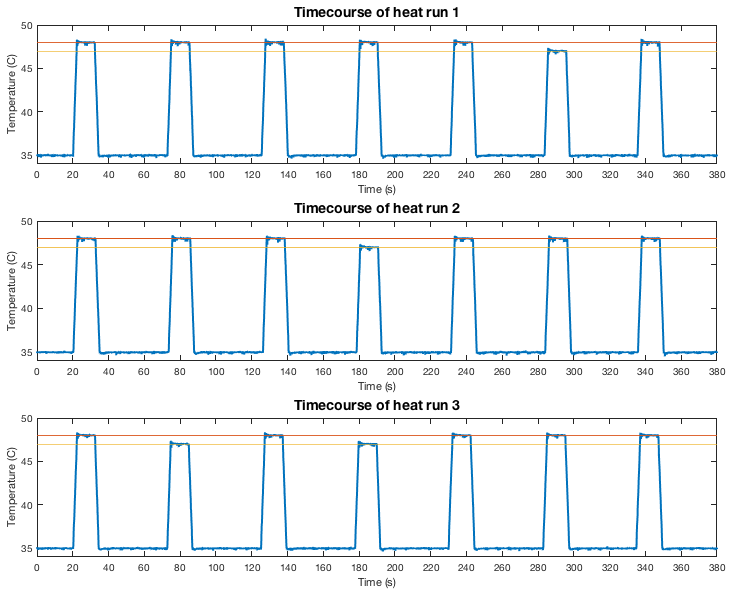
\includegraphics[width=.95\textwidth]{figures/bMethods/Stim_design} 
	 \caption{Illustrations of the time courses of heat stimuli for all three heat runs. The blue graphs depict the temperature of the heat stimuli and the yellow and red lines are used to distinguish between 47 and 48\degree C. In the first heat run the 47\degree C stimulus was delivered as the 6th stimulus, in the second as the 4th stimulus and in the third as the 2nd and 4th stimuli. The remaining stimuli were of 48\degree C.}
	\label{fig:meth:stimdesign} 
\end{figure}

To minimize bias all participants received the same stimuli in a single-blind fashion. Furthermore, the stimuli was induced in a pseudo-random order to confine the effects of habituation and expectation. 
